% Documents setup
\documentclass[11pt]{book}

% fix for pandoc 1.14
\providecommand{\tightlist}{%
  \setlength{\itemsep}{0pt}\setlength{\parskip}{0pt}}

\usepackage{tabu} % https://tex.stackexchange.com/questions/50332/vertical-spacing-of-a-table-cell

% Location of the csas-style repository: adjust path as needed
\newcommand{\locRepo}{csas-style}

% Use the style file in the csas-style repository (res-doc.sty)
\usepackage{\locRepo/res-doc}

% header-includes from R markdown entry


% Headers and footers
\lhead{Draft working paper --- Do not cite or circulate}
% \lhead{}
\rhead{}
% \rfoot{DRAFT - DO NOT CITE}

%%%% Commands for title page etc %%%%%

% Publication year
\newcommand{\rdYear}{2020}

% Publication month
\newcommand{\rdMonth}{}

% Report number
\newcommand{\rdNumber}{nnn}

% Region
\newcommand{\rdRegion}{Pacific Region}

% Title
\newcommand{\rdTitle}{Update to the assessment of Pacific Cod (\emph{Gadus macrocephalus}) for Hecate Strait and Queen Charlotte Sound (Area 5ABCD), and West Coast Vancouver Island (Area 3CD) in 2020}

% Author names separated by commas and ', and' for the last author in the format 'M.H. Grinnell' (use \textsuperscript{n} for addresses)
\newcommand{\rdAuth}{Robyn E. Forrest \ldots{}\textsuperscript{1}}

% Author names reversed separated by commas in the format 'Grinnell, M.H.'
\newcommand{\rdAuthRev}{Forrest, R.E., \ldots{}}

% Author addresses (use \textsuperscript{n})
\newcommand{\rdAuthAddy}{\textsuperscript{1}Pacific Biological Station\\
Fisheries and Oceans Canada, 3190 Hammond Bay Road\\
Nanaimo, British Columbia, V9T 6N7, Canada\\}

\newcommand{\citationOtherLanguage}{}

% Name of file with abstract and resume (see \abstract and \frenchabstract for requirements)
\newcommand{\rdAbstract}{\abstract{The status of two stocks of Pacific Cod (\emph{Gadus macrocephalus}) in Hecate Strait/Queen Charlotte Sound (Area 5ABCD) and West Coast Vancouver Island (Area 3CD) was updated from the 2018 assessment, using Bayesian delay-difference models and data streams updated to 2019. The models were fit to fishery-independent indices of abundance and standardized commercial catch-per-unit-effort (CPUE) indices, updated from the 2018 stock assessment.}}

%%%% End of title page commands %%%%%

% \pdfcompresslevel=5 % faster PNGs

\setcounter{section}{0}

\bibliographystyle{csas-style/res-doc}

\usepackage{amsmath}
\usepackage{bm}

% commands and environments needed by pandoc snippets
% extracted from the output of `pandoc -s`
%% Make R markdown code chunks work
\usepackage{array}
\usepackage{amssymb,amsmath}
\usepackage{color}
\usepackage{fancyvrb}
\DefineShortVerb[commandchars=\\\{\}]{\|}
\DefineVerbatimEnvironment{Highlighting}{Verbatim}{commandchars=\\\{\}}
% Add ',fontsize=\small' for more characters per line
\newenvironment{Shaded}{}{}
\newcommand{\KeywordTok}[1]{\textcolor[rgb]{0.00,0.44,0.13}{\textbf{{#1}}}}
\newcommand{\DataTypeTok}[1]{\textcolor[rgb]{0.56,0.13,0.00}{{#1}}}
\newcommand{\DecValTok}[1]{\textcolor[rgb]{0.25,0.63,0.44}{{#1}}}
\newcommand{\BaseNTok}[1]{\textcolor[rgb]{0.25,0.63,0.44}{{#1}}}
\newcommand{\FloatTok}[1]{\textcolor[rgb]{0.25,0.63,0.44}{{#1}}}
\newcommand{\CharTok}[1]{\textcolor[rgb]{0.25,0.44,0.63}{{#1}}}
\newcommand{\StringTok}[1]{\textcolor[rgb]{0.25,0.44,0.63}{{#1}}}
\newcommand{\CommentTok}[1]{\textcolor[rgb]{0.38,0.63,0.69}{\textit{{#1}}}}
\newcommand{\OtherTok}[1]{\textcolor[rgb]{0.00,0.44,0.13}{{#1}}}
\newcommand{\AlertTok}[1]{\textcolor[rgb]{1.00,0.00,0.00}{\textbf{{#1}}}}
\newcommand{\FunctionTok}[1]{\textcolor[rgb]{0.02,0.16,0.49}{{#1}}}
\newcommand{\RegionMarkerTok}[1]{{#1}}
\newcommand{\ErrorTok}[1]{\textcolor[rgb]{1.00,0.00,0.00}{\textbf{{#1}}}}
\newcommand{\NormalTok}[1]{{#1}}
\newcommand{\OperatorTok}[1]{\textcolor[rgb]{0.00,0.44,0.13}{\textbf{{#1}}}}
\newcommand{\BuiltInTok}[1]{\textcolor[rgb]{0.00,0.44,0.13}{\textbf{{#1}}}}
\newcommand{\ControlFlowTok}[1]{\textcolor[rgb]{0.00,0.44,0.13}{\textbf{{#1}}}}

%Defines cslreferences environment
%Required by pandoc 2.8
%Copied from https://github.com/rstudio/rmarkdown/issues/1649

\DeclareGraphicsExtensions{.png,.pdf}
\begin{document}

\frontmatter
\begin{verbatim}

Attaching package: 'dplyr'
\end{verbatim}
\begin{verbatim}
The following objects are masked from 'package:stats':

    filter, lag
\end{verbatim}
\begin{verbatim}
The following objects are masked from 'package:base':

    intersect, setdiff, setequal, union
\end{verbatim}
\clearpage

\hypertarget{introduction}{%
\section{Introduction}\label{introduction}}

Update to 2018 Pacific Cod assessment (Forrest et al. \protect\hyperlink{ref-forrest2020}{2020}).

\clearpage

\hypertarget{tables}{%
\section{TABLES}\label{tables}}
\begin{longtable}[]{@{}lrrrrr@{}}
\caption{\label{tab:tab-catch-5abcd}Reported catch (mt) of Pacific Cod in Area 5ABCD by Canada and the USA, 1953--2020. The reported discards for the period 1953--1995 are unrepresentative of true discarding because the estimates were taken from logbooks. Discard estimates since 1996 are based on at-sea observations and are considered to be more representative of true discarding.}\tabularnewline
\toprule
\textbf{Year} & \textbf{Canada landed} & \textbf{Canada released at sea} & \textbf{Canada total} & \textbf{USA} & \textbf{Total catch}\tabularnewline
\midrule
\endfirsthead
\toprule
\textbf{Year} & \textbf{Canada landed} & \textbf{Canada released at sea} & \textbf{Canada total} & \textbf{USA} & \textbf{Total catch}\tabularnewline
\midrule
\endhead
1953 & 329 & 0 & 329 & 0 & 329\tabularnewline
1954 & 937 & 0 & 937 & 0 & 937\tabularnewline
1955 & 607 & 0 & 607 & 224 & 831\tabularnewline
1956 & 1,666 & 0 & 1,666 & 2,063 & 3,729\tabularnewline
1957 & 3,199 & 0 & 3,199 & 2,677 & 5,876\tabularnewline
1958 & 3,275 & 0 & 3,275 & 3,549 & 6,824\tabularnewline
1959 & 2,478 & 0 & 2,478 & 1,974 & 4,452\tabularnewline
1960 & 2,029 & 0 & 2,029 & 951 & 2,980\tabularnewline
1961 & 1,529 & 0 & 1,529 & 251 & 1,780\tabularnewline
1962 & 2,138 & 0 & 2,138 & 310 & 2,448\tabularnewline
1963 & 2,478 & 0 & 2,478 & 883 & 3,361\tabularnewline
1964 & 6,568 & 0 & 6,568 & 1,009 & 7,577\tabularnewline
1965 & 9,291 & 0 & 9,291 & 1,562 & 10,853\tabularnewline
1966 & 9,409 & 0 & 9,409 & 1,362 & 10,771\tabularnewline
1967 & 6,034 & 0 & 6,034 & 1,025 & 7,059\tabularnewline
1968 & 4,325 & 0 & 4,325 & 606 & 4,931\tabularnewline
1969 & 2,817 & 0 & 2,817 & 405 & 3,222\tabularnewline
1970 & 1,267 & 0 & 1,267 & 198 & 1,465\tabularnewline
1971 & 1,542 & 0 & 1,542 & 698 & 2,240\tabularnewline
1972 & 3,642 & 0 & 3,642 & 1,667 & 5,309\tabularnewline
1973 & 4,258 & 0 & 4,258 & 1,426 & 5,684\tabularnewline
1974 & 6,005 & 0 & 6,005 & 1,539 & 7,544\tabularnewline
1975 & 6,739 & 0 & 6,739 & 1,139 & 7,878\tabularnewline
1976 & 5,796 & 0 & 5,796 & 635 & 6,431\tabularnewline
1977 & 4,369 & 0 & 4,369 & 408 & 4,777\tabularnewline
1978 & 4,078 & 0 & 4,078 & 159 & 4,237\tabularnewline
1979 & 7,462 & 0 & 7,462 & 62 & 7,524\tabularnewline
1980 & 5,487 & 0 & 5,487 & 10 & 5,497\tabularnewline
1981 & 3,462 & 0 & 3,462 & 0 & 3,462\tabularnewline
1982 & 3,089 & 0 & 3,089 & 0 & 3,089\tabularnewline
1983 & 2,478 & 0 & 2,478 & 0 & 2,478\tabularnewline
1984 & 2,113 & 0 & 2,113 & 0 & 2,113\tabularnewline
1985 & 1,338 & 0 & 1,338 & 0 & 1,338\tabularnewline
1986 & 4,019 & 0 & 4,019 & 0 & 4,019\tabularnewline
1987 & 12,711 & 0 & 12,711 & 0 & 12,711\tabularnewline
1988 & 8,020 & 0 & 8,020 & 0 & 8,020\tabularnewline
1989 & 4,214 & 0 & 4,214 & 0 & 4,214\tabularnewline
1990 & 4,242 & 0 & 4,242 & 0 & 4,242\tabularnewline
1991 & 9,892 & 0 & 9,892 & 0 & 9,892\tabularnewline
1992 & 7,087 & 0 & 7,087 & 0 & 7,087\tabularnewline
1993 & 4,869 & 0 & 4,869 & 0 & 4,869\tabularnewline
1994 & 1,757 & 0 & 1,757 & 0 & 1,757\tabularnewline
1995 & 1,293 & 1 & 1,294 & 0 & 1,294\tabularnewline
1996 & 1,270 & 92 & 1,362 & 0 & 1,362\tabularnewline
1997 & 1,261 & 105 & 1,366 & 0 & 1,366\tabularnewline
1998 & 982 & 59 & 1,041 & 0 & 1,041\tabularnewline
1999 & 692 & 53 & 746 & 0 & 746\tabularnewline
2000 & 553 & 28 & 581 & 0 & 581\tabularnewline
2001 & 296 & 38 & 334 & 0 & 334\tabularnewline
2002 & 382 & 104 & 487 & 0 & 487\tabularnewline
2003 & 660 & 147 & 807 & 0 & 807\tabularnewline
2004 & 833 & 130 & 963 & 0 & 963\tabularnewline
2005 & 1,004 & 83 & 1,087 & 0 & 1,087\tabularnewline
2006 & 872 & 32 & 904 & 0 & 904\tabularnewline
2007 & 370 & 15 & 385 & 0 & 385\tabularnewline
2008 & 309 & 7 & 316 & 0 & 316\tabularnewline
2009 & 669 & 40 & 709 & 0 & 709\tabularnewline
2010 & 1,452 & 49 & 1,501 & 0 & 1,501\tabularnewline
2011 & 1,233 & 7 & 1,240 & 0 & 1,240\tabularnewline
2012 & 871 & 12 & 883 & 0 & 883\tabularnewline
2013 & 829 & 22 & 851 & 0 & 851\tabularnewline
2014 & 904 & 18 & 922 & 0 & 922\tabularnewline
2015 & 924 & 18 & 943 & 0 & 943\tabularnewline
2016 & 529 & 5 & 534 & 0 & 534\tabularnewline
2017 & 346 & 4 & 350 & 0 & 350\tabularnewline
2018 & 254 & 5 & 259 & 0 & 259\tabularnewline
2019 & 450 & 4 & 454 & 0 & 454\tabularnewline
\bottomrule
\end{longtable}
\clearpage
\begin{longtable}[]{@{}lrrrrr@{}}
\caption{\label{tab:tab-catch-3cd}Reported catch (mt) of Pacific Cod in Area 3CD by Canada and the USA, 1953--2020. The reported discards for the period 1953--1995 are unrepresentative of true discarding because the estimates were taken from logbooks. Discard estimates since 1996 are based on at-sea observations and are considered to be more representative of true discarding.}\tabularnewline
\toprule
\textbf{Year} & \textbf{Canada landed} & \textbf{Canada released at sea} & \textbf{Canada total} & \textbf{USA} & \textbf{Total catch}\tabularnewline
\midrule
\endfirsthead
\toprule
\textbf{Year} & \textbf{Canada landed} & \textbf{Canada released at sea} & \textbf{Canada total} & \textbf{USA} & \textbf{Total catch}\tabularnewline
\midrule
\endhead
1953 & 64 & 0 & 64 & 0 & 64\tabularnewline
1954 & 1,055 & 0 & 1,055 & 0 & 1,055\tabularnewline
1955 & 650 & 0 & 650 & 0 & 650\tabularnewline
1956 & 715 & 0 & 715 & 770 & 1,485\tabularnewline
1957 & 1,117 & 0 & 1,117 & 558 & 1,675\tabularnewline
1958 & 526 & 0 & 526 & 271 & 797\tabularnewline
1959 & 416 & 0 & 416 & 510 & 926\tabularnewline
1960 & 240 & 0 & 240 & 376 & 616\tabularnewline
1961 & 284 & 0 & 284 & 232 & 516\tabularnewline
1962 & 428 & 0 & 428 & 402 & 830\tabularnewline
1963 & 838 & 0 & 838 & 345 & 1,183\tabularnewline
1964 & 1,107 & 0 & 1,107 & 907 & 2,014\tabularnewline
1965 & 1,608 & 0 & 1,608 & 1,088 & 2,696\tabularnewline
1966 & 2,095 & 0 & 2,095 & 1,145 & 3,240\tabularnewline
1967 & 1,202 & 0 & 1,202 & 623 & 1,825\tabularnewline
1968 & 726 & 0 & 726 & 351 & 1,077\tabularnewline
1969 & 796 & 0 & 796 & 147 & 943\tabularnewline
1970 & 1,150 & 0 & 1,150 & 454 & 1,604\tabularnewline
1971 & 3,585 & 0 & 3,585 & 1,319 & 4,904\tabularnewline
1972 & 4,447 & 0 & 4,447 & 1,271 & 5,718\tabularnewline
1973 & 2,457 & 0 & 2,457 & 627 & 3,084\tabularnewline
1974 & 2,913 & 0 & 2,913 & 1,013 & 3,926\tabularnewline
1975 & 2,854 & 0 & 2,854 & 1,359 & 4,213\tabularnewline
1976 & 2,187 & 0 & 2,187 & 1,679 & 3,866\tabularnewline
1977 & 1,608 & 0 & 1,608 & 1,344 & 2,952\tabularnewline
1978 & 1,168 & 0 & 1,168 & 1,086 & 2,254\tabularnewline
1979 & 1,530 & 0 & 1,530 & 741 & 2,271\tabularnewline
1980 & 1,117 & 0 & 1,117 & 287 & 1,404\tabularnewline
1981 & 1,518 & 0 & 1,518 & 0 & 1,518\tabularnewline
1982 & 608 & 0 & 608 & 0 & 608\tabularnewline
1983 & 883 & 0 & 883 & 0 & 883\tabularnewline
1984 & 506 & 0 & 506 & 0 & 506\tabularnewline
1985 & 440 & 0 & 440 & 0 & 440\tabularnewline
1986 & 441 & 0 & 441 & 0 & 441\tabularnewline
1987 & 1,400 & 0 & 1,400 & 0 & 1,400\tabularnewline
1988 & 3,153 & 0 & 3,153 & 0 & 3,153\tabularnewline
1989 & 1,958 & 0 & 1,958 & 0 & 1,958\tabularnewline
1990 & 2,076 & 0 & 2,076 & 0 & 2,076\tabularnewline
1991 & 2,971 & 0 & 2,971 & 0 & 2,971\tabularnewline
1992 & 2,229 & 0 & 2,229 & 0 & 2,229\tabularnewline
1993 & 2,091 & 0 & 2,091 & 0 & 2,091\tabularnewline
1994 & 816 & 0 & 816 & 0 & 816\tabularnewline
1995 & 252 & 1 & 253 & 0 & 253\tabularnewline
1996 & 146 & 9 & 155 & 0 & 155\tabularnewline
1997 & 135 & 10 & 145 & 0 & 145\tabularnewline
1998 & 56 & 5 & 61 & 0 & 61\tabularnewline
1999 & 75 & 8 & 83 & 0 & 83\tabularnewline
2000 & 129 & 13 & 142 & 0 & 142\tabularnewline
2001 & 342 & 16 & 358 & 0 & 358\tabularnewline
2002 & 177 & 26 & 204 & 0 & 204\tabularnewline
2003 & 458 & 41 & 499 & 0 & 499\tabularnewline
2004 & 418 & 27 & 444 & 0 & 444\tabularnewline
2005 & 265 & 29 & 294 & 0 & 294\tabularnewline
2006 & 143 & 10 & 153 & 0 & 153\tabularnewline
2007 & 55 & 13 & 68 & 0 & 68\tabularnewline
2008 & 105 & 7 & 111 & 0 & 111\tabularnewline
2009 & 365 & 56 & 421 & 0 & 421\tabularnewline
2010 & 577 & 25 & 602 & 0 & 602\tabularnewline
2011 & 503 & 9 & 512 & 0 & 512\tabularnewline
2012 & 399 & 19 & 418 & 0 & 418\tabularnewline
2013 & 361 & 29 & 389 & 0 & 389\tabularnewline
2014 & 442 & 12 & 454 & 0 & 454\tabularnewline
2015 & 445 & 3 & 449 & 0 & 449\tabularnewline
2016 & 323 & 2 & 325 & 0 & 325\tabularnewline
2017 & 164 & 1 & 164 & 0 & 164\tabularnewline
2018 & 23 & 0 & 23 & 0 & 23\tabularnewline
2019 & 43 & 4 & 47 & 0 & 47\tabularnewline
\bottomrule
\end{longtable}
\clearpage
\begin{longtable}[]{@{}lrrrrl@{}}
\caption{\label{tab:tab-tac}Summary of TACs by area.}\tabularnewline
\toprule
\textbf{Year} & \textbf{3CD} & \textbf{5AB} & \textbf{5CDE} & \textbf{Total} & \textbf{Source}\tabularnewline
\midrule
\endfirsthead
\toprule
\textbf{Year} & \textbf{3CD} & \textbf{5AB} & \textbf{5CDE} & \textbf{Total} & \textbf{Source}\tabularnewline
\midrule
\endhead
2018-19 & 500 & 250 & 700 & 1,450 & IFMP\tabularnewline
2017-18 & 500 & 250 & 700 & 1,450 & IFMP\tabularnewline
2016-17 & 500 & 200 & 700 & 1,400 & IFMP\tabularnewline
2015-16 & 500 & 400 & 1,200 & 2,100 & IFMP\tabularnewline
2014-15 & 500 & 590 & 1,200 & 2,290 & IFMP\tabularnewline
2013-14 & 500 & 590 & 1,200 & 2,290 & IFMP\tabularnewline
2012-13 & 500 & 590 & 1,200 & 2,290 & IFMP\tabularnewline
2011-12 & 500 & 590 & 1,200 & 2,290 & IFMP\tabularnewline
2010-11 & 500 & 390 & 800 & 1,690 & IFMP\tabularnewline
2009-10 & 500 & 390 & 800 & 1,690 & IFMP\tabularnewline
2008-09 & 500 & 390 & 800 & 1,690 & IFMP\tabularnewline
2007-08 & 500 & 390 & 800 & 1,690 & IFMP\tabularnewline
2006-07 & 500 & 390 & 800 & 1,690 & IFMP\tabularnewline
2005-06 & 500 & 390 & 800 & 1,690 & GMU Trawl TAC xls\tabularnewline
2004-05 & 500 & 390 & 400 & 1,290 & GMU Trawl TAC xls\tabularnewline
2003-04 & 500 & 260 & 400 & 1,160 & GMU Trawl TAC xls\tabularnewline
2002-03 & 240 & 260 & 200 & 700 & GMU Trawl TAC xls\tabularnewline
2001-02 & 694 & 260 & 200 & 1,154 & GMU Trawl TAC xls\tabularnewline
2000-01 & 694 & 260 & 1,000 & 1,954 & GMU Trawl TAC xls\tabularnewline
1999-00 & 694 & 260 & 1,000 & 1,954 & GMU Trawl TAC xls\tabularnewline
1998-99 & 694 & 260 & 1,000 & 1,954 & GMU Trawl TAC xls\tabularnewline
1997-98 & 694 & 260 & 1,620 & 2,574 & GMU Trawl TAC xls\tabularnewline
1996-97 & bycatch only & bycatch only & bycatch only & 0 & CSAS ResDoc 2015/052\tabularnewline
\bottomrule
\end{longtable}
\clearpage

\clearpage
\begin{longtable}[]{@{}lll@{}}
\caption{\label{tab:tab-suggested-ref-points}Reference points for the Reference Case 5ABCD and 3CD models.}\tabularnewline
\toprule
\textbf{Reference point} & \textbf{Definition} & \textbf{Role}\tabularnewline
\midrule
\endfirsthead
\toprule
\textbf{Reference point} & \textbf{Definition} & \textbf{Role}\tabularnewline
\midrule
\endhead
\(B_{ {Min}}\) & \mlc{Lowest estimated biomass agreed to be an \\ undesirable state to avoid ($B_{	{2000}}$ \\ in  5ABCD; $B_{	{1986}}$ in 3CD)} & LRP\tabularnewline
\(B_{ {Avg}}\) & Average biomass for the period 1956-2004 & USR\tabularnewline
\(F_{ {Avg}}\) & Average fishing mortality for the period 1956-2004 & LRR\tabularnewline
\(B_{ {2018}}\) & Biomass in 2018 & Benchmark\tabularnewline
\(F_{ {2017}}\) & Fishing mortality in 2017 & Benchmark\tabularnewline
\bottomrule
\end{longtable}
\clearpage

\hypertarget{model-results-area-5abcd}{%
\subsection{MODEL RESULTS: AREA 5ABCD}\label{model-results-area-5abcd}}

\clearpage

\clearpage

\clearpage

\clearpage

\hypertarget{model-results-area-3cd}{%
\subsection{MODEL RESULTS: AREA 3CD}\label{model-results-area-3cd}}

\clearpage

\clearpage

\clearpage

\clearpage

\hypertarget{selected-sensitivity-results}{%
\subsection{SELECTED SENSITIVITY RESULTS}\label{selected-sensitivity-results}}

\emph{Copy Sensitivity chunks from 2018 Rmd file if needed}

\clearpage

\hypertarget{sec:reference-points-and-decision-tables}{%
\subsection{MODEL-AVERAGED REFERENCE POINTS AND DECISION TABLES}\label{sec:reference-points-and-decision-tables}}

\vspace{10pt}

\clearpage

\clearpage

\Appendices


\clearpage

\refstepcounter{chapter}
\hypertarget{fishery-independent-indices-of-abundance}{%
\starredchapter{APPENDIX~\thechapter. FISHERY-INDEPENDENT INDICES OF ABUNDANCE}\label{fishery-independent-indices-of-abundance}}

\hypertarget{canadian-surveys}{%
\appsection{CANADIAN SURVEYS}\label{canadian-surveys}}

\hypertarget{hecate-strait-assemblage-survey}{%
\subsection{HECATE STRAIT ASSEMBLAGE SURVEY}\label{hecate-strait-assemblage-survey}}

A series of multi-species groundfish bottom trawl surveys was conducted in Hecate Strait in May-June of 1984, 1987, 1989, 1991, 1993, 1995, 1996, 1998, 2000, 2002, and 2003 Westrheim et al. (\protect\hyperlink{ref-westrheim1984}{1984}), Fargo et al. (\protect\hyperlink{ref-fargo1984}{1984}), Fargo et al. (\protect\hyperlink{ref-fargo1988}{1988}), Wilson et al. (\protect\hyperlink{ref-wilson1991}{1991}), Hand et al. (\protect\hyperlink{ref-hand1994}{1994}), Workman et al. (\protect\hyperlink{ref-workman1996}{1996}), Workman et al. (\protect\hyperlink{ref-workman1997}{1997}), Choromanski et al. (\protect\hyperlink{ref-choromanski2002}{2002})) (Figure~\ref{fig:survey-maps-hs-msa}. The results up to 2000 were reported in the 2001 assessment (Sinclair et al. \protect\hyperlink{ref-sinclair2001}{2001}) and results from 2002 and 2003 were presented in the 2005 assessment (Sinclair and Starr \protect\hyperlink{ref-sinclair2005}{2005}).

The original design of this survey assigned fishing locations by 10 fm depth intervals within a 10 nm grid of Hecate Strait. The survey was post-stratified for the purpose of calculating an abundance index for Pacific Cod (Sinclair \protect\hyperlink{ref-sinclair2000}{1999}). The post stratification used 10 fm depth intervals for the entire survey area, thereby treating each depth interval as a single stratum.

The Hecate Strait Assemblage survey was designed as a systematic fixed-station survey. Despite attempts to apply post-sampling stratification, this approach had high survey variance (Sinclair et al. \protect\hyperlink{ref-sinclair2007}{2007}). In 2004 the Hecate Strait Assemblage survey was discontinued in favour of the Hecate Strait Synoptic survey (described below).

\hypertarget{hecate-strait-synoptic-survey}{%
\subsection{HECATE STRAIT SYNOPTIC SURVEY}\label{hecate-strait-synoptic-survey}}

The Hecate Strait synoptic groundfish bottom trawl survey is part of a coordinated set of long-term surveys that together cover the continental shelf and upper slope of most of the BC coast (Figure~\ref{fig:survey-maps-syn-hs}. The Hecate Strait synoptic survey has been conducted during May-June, in odd years since 2005. All the synoptic surveys follow a random depth stratified design. The survey area is divided into 2 km by 2 km blocks and each block is assigned to one of four depth strata based on the average bottom depth in the block. The four depth strata for the Hecate Strait survey are 10--70m, 70--130m, 130--220m, and 220--500m. Each year blocks are randomly selected within each depth strata. For this survey and the other synoptic surveys discussed below, the relative allocation of blocks amongst depth strata was determined by modeling the expected catches of groundfish and determining the target number of tows per stratum that would provide sufficiently precise catch rate data for as many species as possible.

\hypertarget{queen-charlotte-sound-synoptic-survey}{%
\subsection{QUEEN CHARLOTTE SOUND SYNOPTIC SURVEY}\label{queen-charlotte-sound-synoptic-survey}}

The Queen Charlotte Sound (QCS) synoptic groundfish bottom trawl survey has been conducted in July--August in 2003, 2004, and in odd years since 2005 (Figure~\ref{fig:survey-maps-syn-qcs}. The four depth strata for the QCS survey are 50--125m, 125--200m, 200--330m, and 330--500 m. Each year blocks are randomly selected within each depth strata. In addition, for the purposes of allocating blocks, the QCS survey is divided into northern and southern spatial strata.

\hypertarget{west-coast-vancouver-island-synoptic-survey}{%
\subsection{WEST COAST VANCOUVER ISLAND SYNOPTIC SURVEY}\label{west-coast-vancouver-island-synoptic-survey}}

The West Coast Vancouver Island synoptic bottom trawl survey was first conducted in 2004 and is conducted in alternating (even-numbered) years on a chartered commercial trawler (Figure~\ref{fig:survey-maps-syn-wcvi}). The survey area is off the west coast of Vancouver Island from approximately 49 \(^\circ\) 12\(^\prime\) to 50 \(^\circ\) 36\(^\prime\) North latitude and approximately 124 \(^\circ\) 48\(^\prime\) to 128 \(^\circ\) 30\(^\prime\) West longitude. The southern boundary is contiguous with the Canada/U.S. boundary. The survey has a single aerial stratum in Pacific Fishery Management Area regions 3C and 3D separated into four depth strata: 50--125m; 125--200m; 200--330m; and 330--500m. Approximately 150 to 180 4 km\textsuperscript{2} blocks are selected randomly among the four depth strata when conducting each survey.
\begin{figure}[htb]

{\centering \pdftooltip{\includegraphics[width=6in]{knitr-figs/survey-maps-hs-msa-1}}{Figure \ref{fig:survey-maps-hs-msa}} 

}

\caption{Individual survey tows for the Hecate Strait multi-species groundfish bottom trawl survey. Light gray crosses indicate survey sets that did not catch Pacific Cod. Circles have their area and color proportional to the density of Pacific Cod for that survey set. Eastings and Northings are for UTM zone 9.}\label{fig:survey-maps-hs-msa}
\end{figure}
\begin{figure}[htb]

{\centering \pdftooltip{\includegraphics[width=6in]{knitr-figs/survey-maps-syn-hs-1}}{Figure \ref{fig:survey-maps-syn-hs}} 

}

\caption{Individual survey tows for the Hecate Strait (SYN HS) synoptic groundfish bottom trawl survey. Light gray crosses indicate survey sets that did not catch Pacific Cod. Circles have their area and color proportional to the density of Pacific Cod for that survey set. Eastings and Northings are for UTM zone 9.}\label{fig:survey-maps-syn-hs}
\end{figure}
\begin{figure}[htb]

{\centering \pdftooltip{\includegraphics[width=6in]{knitr-figs/survey-maps-syn-qcs-1}}{Figure \ref{fig:survey-maps-syn-qcs}} 

}

\caption{Individual survey tows for the Queen Charlotte Sound (SYN QCS) synoptic groundfish bottom trawl survey. Light gray crosses indicate survey sets that did not catch Pacific Cod. Circles have their area and color proportional to the density of Pacific Cod for that survey set. Eastings and Northings are for UTM zone 9.}\label{fig:survey-maps-syn-qcs}
\end{figure}
\begin{figure}[htb]

{\centering \pdftooltip{\includegraphics[width=6in]{knitr-figs/survey-maps-syn-wcvi-1}}{Figure \ref{fig:survey-maps-syn-wcvi}} 

}

\caption{Individual survey tows for the West Coast Vancouver Island (SYN WCVI) synoptic groundfish bottom trawl survey survey. Light gray crosses indicate survey sets that did not catch Pacific Cod. Circles have their area and color proportional to the density of Pacific Cod for that survey set. Eastings and Northings are for UTM zone 9.}\label{fig:survey-maps-syn-wcvi}
\end{figure}
\clearpage

\hypertarget{swept-area-analysis}{%
\subsection{SWEPT AREA ANALYSIS}\label{swept-area-analysis}}

For all Canadian surveys, a swept area estimate of biomass in any year \(y\) was obtained by summing the product of the CPUE and the area surveyed across the surveyed strata \(i\):
\begin{equation}
  B_y = \sum_{i=1}^kC_{y_i}A_i=\sum_{i=1}^kB_{y_i}
  \label{eq:sweptareabiomass}
\end{equation}
where \(C_{y_i}\) = mean CPUE density (kg/km\textsuperscript{2}) for Pacific Cod in stratum \(i\), \(A_i\) = area of stratum \(i\) (km\textsuperscript{2}), \(B_{y_i}\) = biomass of Pacific Cod in stratum \(i\) for year \(y\), and \(k\) = number of strata.

CPUE (\(C_{y_i}\)) for Pacific Cod in stratum \(i\) for year \(y\) was calculated as a density in kg/km\textsuperscript{2} by
\begin{equation}
  C_{y_i}=\frac{1}{n_{y_i}} \sum\limits_{j=1}^{n_{y_i}} \frac{W_{y_i,j}}{D_{y_i,j}w_{y_i,j}}
  \label{eq:sweptareacpue}
\end{equation}
where \(W_{y_i,j}\) = catch weight (kg) for Pacific Cod in stratum \(i\) for year \(y\) and tow \(j\), \(D_{y_i,j}\) = distance travelled (km) by tow \(j\) in stratum \(i\) for year \(y\), \(w_{y_i,j}\) = net opening (km) by tow \(j\) in stratum \(i\) for year \(y\), and \(n_{y_i}\) = number of tows in stratum \(i\).

The variance of the survey biomass estimate \(V_y\) for Pacific Cod in year \(y\) was calculated in kg\textsuperscript{2} as follows:
\begin{equation}
  V_y=\sum_{i=1}^k\frac{\sigma_{y_i}^2A_i^2}{n_{y_i}}=\sum_{i=1}^kV_{y_i}
  \label{eq:sweptareavariance}
\end{equation}
where \(\sigma_{y_i}^2\) is the variance of the CPUE in \(kg^2/km^4\) for year \(y\) in stratum \(i\), \(V_{y_i}\) is the variance of Pacific Cod in stratum \(i\) for year \(y\), and where \(\sigma_{y_i}^2\) was obtained from bootstrapped samples (see below).

The CV for Pacific Cod for each year \(y\) was calculated as follows:
\begin{equation}
  (CV)_y=\frac{{V_y}^{1/2}}{B_y}
  \label{eq:sweptareacv}
\end{equation}
where \((CV)_y\) is the CV for year \(y\).

One thousand bootstrap replicates with replacement were constructed from the survey data to estimate bias corrected 95\% confidence intervals for each survey year (Efron \protect\hyperlink{ref-efron1982}{1982}). The resulting values are shown in Table~\ref{tab:surv-canadian-table} and Figure~\ref{fig:surv-canadian}.
\begin{longtable}[]{@{}lrrrrrrr@{}}
\caption{\label{tab:surv-canadian-table}Pacific Cod survey data for Canadian trawl surveys. Relative biomass and associated lower and upper confidence intervals (CI) are shown in metric tons (without accounting for survey catchability). Positive sets refers to the number of trawl sets that caught Pacific Cod.}\tabularnewline
\toprule
Survey abbrev. & Year & Biomass & CV & Lower CI & Upper CI & Sets & Positive sets\tabularnewline
\midrule
\endfirsthead
\toprule
Survey abbrev. & Year & Biomass & CV & Lower CI & Upper CI & Sets & Positive sets\tabularnewline
\midrule
\endhead
OTHER HS MSA & 1984 & 1142.4 & 0.30 & 606.6 & 1929.9 & 146 & 88\tabularnewline
OTHER HS MSA & 1987 & 3875.7 & 0.35 & 1501.2 & 6778.9 & 85 & 43\tabularnewline
OTHER HS MSA & 1989 & 4102.8 & 0.43 & 1318.5 & 7976.0 & 90 & 48\tabularnewline
OTHER HS MSA & 1991 & 1031.8 & 0.30 & 506.1 & 1679.0 & 97 & 59\tabularnewline
OTHER HS MSA & 1993 & 1255.6 & 0.24 & 719.9 & 1862.4 & 94 & 40\tabularnewline
OTHER HS MSA & 1995 & 1419.8 & 0.46 & 528.7 & 2880.5 & 101 & 52\tabularnewline
OTHER HS MSA & 1996 & 1418.5 & 0.26 & 793.2 & 2208.0 & 158 & 83\tabularnewline
OTHER HS MSA & 1998 & 4253.0 & 0.51 & 1223.7 & 9186.9 & 86 & 52\tabularnewline
OTHER HS MSA & 2000 & 436.1 & 0.20 & 283.7 & 622.8 & 105 & 54\tabularnewline
OTHER HS MSA & 2002 & 2025.9 & 0.27 & 1137.3 & 3203.6 & 91 & 66\tabularnewline
OTHER HS MSA & 2003 & 1288.7 & 0.21 & 808.3 & 1871.8 & 95 & 77\tabularnewline
SYN HS & 2005 & 1946.4 & 0.24 & 1192.6 & 2992.5 & 198 & 161\tabularnewline
SYN HS & 2007 & 586.6 & 0.22 & 359.5 & 856.2 & 132 & 72\tabularnewline
SYN HS & 2009 & 2460.8 & 0.45 & 744.7 & 4918.3 & 155 & 102\tabularnewline
SYN HS & 2011 & 1860.7 & 0.26 & 1083.4 & 2978.7 & 184 & 124\tabularnewline
SYN HS & 2013 & 2326.5 & 0.24 & 1443.3 & 3512.3 & 175 & 132\tabularnewline
SYN HS & 2015 & 956.6 & 0.21 & 598.9 & 1394.0 & 148 & 107\tabularnewline
SYN HS & 2017 & 1554.4 & 0.34 & 754.4 & 2792.0 & 138 & 107\tabularnewline
SYN HS & 2019 & 1752.1 & 0.37 & 832.3 & 3204.5 & 136 & 102\tabularnewline
SYN QCS & 2003 & 806.6 & 0.17 & 568.1 & 1092.1 & 233 & 101\tabularnewline
SYN QCS & 2004 & 1624.4 & 0.26 & 901.8 & 2550.5 & 230 & 118\tabularnewline
SYN QCS & 2005 & 1505.0 & 0.35 & 785.6 & 2705.1 & 224 & 125\tabularnewline
SYN QCS & 2007 & 434.5 & 0.25 & 245.5 & 665.9 & 255 & 105\tabularnewline
SYN QCS & 2009 & 565.5 & 0.24 & 335.1 & 859.5 & 233 & 95\tabularnewline
SYN QCS & 2011 & 1018.4 & 0.21 & 644.6 & 1473.9 & 251 & 98\tabularnewline
SYN QCS & 2013 & 928.3 & 0.15 & 680.9 & 1232.9 & 240 & 134\tabularnewline
SYN QCS & 2015 & 1122.3 & 0.29 & 644.0 & 1852.9 & 238 & 124\tabularnewline
SYN QCS & 2017 & 521.8 & 0.17 & 355.2 & 706.0 & 240 & 90\tabularnewline
SYN QCS & 2019 & 1004.0 & 0.13 & 782.6 & 1283.6 & 242 & 113\tabularnewline
SYN WCHG & 2006 & 50.7 & 0.23 & 30.6 & 75.7 & 110 & 36\tabularnewline
SYN WCHG & 2007 & 33.0 & 0.42 & 10.4 & 62.9 & 111 & 23\tabularnewline
SYN WCHG & 2008 & 12.4 & 0.27 & 6.4 & 19.8 & 118 & 20\tabularnewline
SYN WCHG & 2010 & 21.4 & 0.46 & 7.6 & 43.9 & 129 & 27\tabularnewline
SYN WCHG & 2012 & 39.8 & 0.31 & 19.8 & 68.6 & 130 & 34\tabularnewline
SYN WCHG & 2016 & 30.4 & 0.16 & 21.2 & 41.2 & 111 & 41\tabularnewline
SYN WCHG & 2018 & 20.1 & 0.25 & 11.2 & 31.3 & 119 & 22\tabularnewline
SYN WCVI & 2004 & 1133.1 & 0.22 & 696.4 & 1652.4 & 89 & 54\tabularnewline
SYN WCVI & 2006 & 1156.0 & 0.22 & 689.1 & 1693.5 & 164 & 88\tabularnewline
SYN WCVI & 2008 & 512.6 & 0.40 & 233.1 & 986.2 & 159 & 65\tabularnewline
SYN WCVI & 2010 & 1577.4 & 0.17 & 1087.3 & 2128.2 & 136 & 100\tabularnewline
SYN WCVI & 2012 & 921.3 & 0.18 & 626.2 & 1279.6 & 151 & 94\tabularnewline
SYN WCVI & 2014 & 2149.4 & 0.20 & 1342.7 & 3076.3 & 146 & 110\tabularnewline
SYN WCVI & 2016 & 2026.8 & 0.19 & 1325.7 & 2877.8 & 140 & 99\tabularnewline
SYN WCVI & 2018 & 552.9 & 0.21 & 362.3 & 805.9 & 190 & 91\tabularnewline
\bottomrule
\end{longtable}
\begin{figure}[htb]

{\centering \pdftooltip{\includegraphics[width=6in]{knitr-figs/surv-canadian-1}}{Figure \ref{fig:surv-canadian}} 

}

\caption{Pacific Cod survey data for Canadian trawl surveys. Shown is relative biomass and associated lower and upper confidence intervals. Positive sets refers to the number of trawl sets that caught Pacific Cod.}\label{fig:surv-canadian}
\end{figure}
\clearpage

\hypertarget{nmfs-triennial-survey-in-canadian-waters}{%
\appsection{NMFS TRIENNIAL SURVEY (IN CANADIAN WATERS)}\label{nmfs-triennial-survey-in-canadian-waters}}

A relative abundance index was developed for Area 3CD from data from the National Marine Fisheries Service (NMFS) Triennial survey operated off the lower half of Vancouver Island.

\hypertarget{data-selection}{%
\subsection{Data selection}\label{data-selection}}

Tow-by-tow data from the US National Marine Fisheries Service (NMFS) triennial survey covering the Vancouver INPFC (International North Pacific Fisheries Commission) region were provided by Mark Wilkins (NMFS, pers. comm.) for the seven years that the survey worked in BC waters (Table~\ref{tab:surv-tri-strata-table}, Figure~\ref{fig:tri-tows})). These tows were assigned to strata by the NMFS, although the size and definition of these strata have changed over the life of the survey. The NMFS survey database also identified in which country the tow was located. This information was plotted and checked against the accepted Canada/USA marine boundary: all tows appeared to be appropriately located with respect to country, based on the tow start position Figure~\ref{fig:tri-tows})). The NMFS designations were accepted for tows located near the marine border.

All usable tows had an associated median net width (with 1--99\% quantiles) of 13.4 (11.3-15.7) m and median distance travelled of 2.8 (1.4--3.5) km, allowing for the calculation of the area swept by each tow. Biomass indices and the associated analytical CVs for Pacific Cod were calculated for the total Vancouver INPFC region and for each of the Canadian- and US-Vancouver sub-regions, using appropriate area estimates for each stratum and year. Strata that were not surveyed consistently in all seven years of the survey were dropped from the analysis, allowing the remaining data to provide a comparable set of data for each year.
\begin{longtable}[]{@{}lllllllllllllll@{}}
\caption{\label{tab:surv-tri-strata-table}Number of tows by stratum and by survey year for the NFMS triennial survey. Strata denoted with an asterisk have been excluded from the analysis due to incomplete coverage across the seven survey years or were from locations outside the Vancouver INPFC area.}\tabularnewline
\toprule
Stratum No. & 1980 & 1980 & 1983 & 1983 & 1989 & 1989 & 1992 & 1992 & 1995 & 1995 & 1998 & 1998 & 2001 & 2001\tabularnewline
\midrule
\endfirsthead
\toprule
Stratum No. & 1980 & 1980 & 1983 & 1983 & 1989 & 1989 & 1992 & 1992 & 1995 & 1995 & 1998 & 1998 & 2001 & 2001\tabularnewline
\midrule
\endhead
& CDN & US & CDN & US & CDN & US & CDN & US & CDN & US & CDN & US & CDN & US\tabularnewline
10 & & 15 & & 7 & & & & & & & & & &\tabularnewline
11 & 38 & & & 34 & & & & & & & & & &\tabularnewline
12 & & & 32 & & & & & & & & & & &\tabularnewline
17N & & & & & & 8 & & 9 & & 8 & & 8 & & 8\tabularnewline
17S* & & & & & & 27 & & 27 & & 24 & & 26 & & 25\tabularnewline
18N* & & & & & 1 & & 1 & & & & & & &\tabularnewline
18S & & & & & & 31 & & 20 & & 12 & & 20 & & 14\tabularnewline
19N & & & & & 56 & & 53 & & 55 & & 48 & & 33 &\tabularnewline
19S & & & & & & 4 & & 6 & & 3 & & 3 & & 3\tabularnewline
27N & & & & & & 2 & & 1 & & 2 & & 2 & & 2\tabularnewline
27S* & & & & & & 4 & & 2 & & 3 & & 4 & & 5\tabularnewline
28N* & & & & & 1 & & 1 & & 2 & & 1 & & &\tabularnewline
28S & & & & & & 6 & & 9 & & 7 & & 6 & & 7\tabularnewline
29N & & & & & 7 & & 6 & & 7 & & 6 & & 3 &\tabularnewline
29S & & & & & & 3 & & 2 & & 3 & & 3 & & 3\tabularnewline
30 & & 4 & & 2 & & & & & & & & & &\tabularnewline
31 & 7 & & & 11 & & & & & & & & & &\tabularnewline
32 & & & 5 & & & & & & & & & & &\tabularnewline
37N* & & & & & & & & & & 1 & & 1 & & 1\tabularnewline
37S* & & & & & & & & & & 2 & & 1 & & 1\tabularnewline
38N* & & & & & & & & & 1 & & & & &\tabularnewline
38S* & & & & & & & & & & 2 & & & & 3\tabularnewline
39* & & & & & & & & & 6 & & 4 & & 2 &\tabularnewline
50 & & 4 & & 1 & & & & & & & & & &\tabularnewline
51 & 3 & & & 10 & & & & & & & & & &\tabularnewline
52 & & & 2 & & & & & & & & & & &\tabularnewline
Total & 48 & 23 & 39 & 65 & 65 & 85 & 61 & 76 & 71 & 67 & 59 & 74 & 38 & 72\tabularnewline
\bottomrule
\end{longtable}
The stratum definitions used in the 1980 and 1983 surveys were different than those used in subsequent surveys, particularly in Canadian waters. Consequently, these indices were not used in the 3CD stock assessment. The tow density was much higher in US waters although the overall number of tows was approximately the same for each country. This occurs because the size of the total area fished in the INPFC Vancouver area was about twice as large in Canadian waters than in US waters. Note that the northern extension of the survey has varied from year to year (Figure~\ref{fig:tri-tows}), but this difference has been compensated for by using a constant survey area for all years and assuming that catch rates in the unsampled areas were the same as in the sampled area.

A reviewer from NOAA for Yellowtail Rockfish in 2014 noted that a number of the early Triennial survey tows had been deemed ``water hauls'' (catching no fish or invertebrates) and should be discarded. The tows used to estimate relative Pacific Cod biomass exclude these water haul tows.

\hypertarget{triennial-survey-methods}{%
\subsection{TRIENNIAL SURVEY METHODS}\label{triennial-survey-methods}}

When calculating the variance for this survey, it was assumed that the variance and CPUE within any stratum were equal, even for strata that were split by the Canada/USA border. The total biomass within a stratum that straddled the border was split between the two countries by the ratio of the relative area within each country:
\begin{equation}
B_{y_{i,c}}=B_{y_{i}}\frac{A_{y_{i,c}}}{A_{y_{i}}}
\label{eq:tri1}
\end{equation}
where \(A_{y_{i,c}} =\) area (km\textsuperscript{2}) within country \emph{c} in year \emph{y} and stratum \emph{i} and \emph{B} represents biomass.

The variance \emph{V} for that part of stratum \emph{i} within country \emph{c} was calculated as being in proportion to the ratio of the square of the area within each country \emph{c} relative to the total area of stratum \emph{i}. This assumption resulted in the CVs within each country stratum being the same as the CV in the entire stratum:
\begin{equation}
V_{y_{i,c}}=V_{y_{i}}\frac{A_{y_{i,c}}^{2}}{A_{y_{i}}^{2}}.
\label{eq:tri2}
\end{equation}
The partial variance for country \emph{c} was used in instead of the total variance in the stratum when calculating the variance for the total biomass in Canadian or American waters.

The biomass estimates and the associated standard errors were adjusted to a constant area covered using the ratios of area surveyed. This was required to adjust the Canadian biomass estimates for 1980 and 1983 to account for the smaller area surveyed in those years compared to the succeeding surveys. he 1980 and 1983 biomass estimates from Canadian waters were consequently multiplied by the ratio 1.24 (= 9166 km\textsuperscript{2} / 7399 km\textsuperscript{2}) to make them equivalent to the coverage of the surveys from 1989 onwards.

Biomass estimates were bootstrapped for 1000 random draws with replacement to obtain bias-corrected (Efron \protect\hyperlink{ref-efron1982}{1982}) 95\% confidence intervals for each year and for three area categories (total Vancouver region, Canadian-Vancouver only and US-Vancouver only) based on the distribution of biomass estimates and using the above equations.

Catch and effort data for strata \(i\) in year \(y\) yield catch per unit effort (CPUE) values\({U_{yi}}\). Given a set of data \(\left\{ {{C_{yij}},{E_{yij}}} \right\}\) for tows\(j = 1, \ldots ,{n_{yi}}\),
\begin{equation}
{U_{yi}} = \frac{1}{{{n_{yi}}}}\sum\limits_{j = 1}^{{n_{yi}}} {\frac{{{C_{yij}}}}{{{E_{yij}}}}},
\end{equation}
where \({C_{yij}}\) = catch (kg) in tow \(j\), stratum \(i\), year \(y\); \({E_{yij}}\) = effort (h) in tow \(j\), stratum \(i\), year \(y\); and \({n_{yi}}\) = number of tows in stratum \(i\), year \(y\).

CPUE values \({U_{yi}}\) convert to CPUE densities \({\delta _{yi}}\) (kg/km2) using:
\begin{equation}
{\delta _{yi}} = \frac{1}{{vw}}{U_{yi}},
\end{equation}
where \(v\) = average vessel speed (km/h) and \(w\) = average net width (km).

Alternatively, if vessel information exists for every tow, CPUE density can be expressed
\begin{equation}
{\delta _{yi}} = \frac{1}{{{n_{yi}}}}\,\,\sum\limits_{j = 1}^{{n_{yi}}} {\,\frac{{{C_{yij}}}}{{{D_{yij}}{w_{yij}}}}},
\end{equation}
where \({C_{yij}}\) = catch weight (kg) for tow \(j\), stratum \(i\), year \(y\); \({D_{yij}}\) = distance travelled (km) for tow\(j\), stratum\(i\), year\(y\); \({w_{yij}}\) = net opening (km) for tow\(j\), stratum\(i\), year\(y\); and \({n_{yi}}\) = number of tows in stratum\(i\), year\(y\).

The annual biomass estimate is then the sum of the product of CPUE densities and bottom areas across \(m\) strata:
\begin{equation}
{B_y} = \sum\limits_{i = 1}^m {{\delta _{yi}}{A_i}}  = \sum\limits_{i = 1}^m {{B_{yi}}},
\end{equation}
where \({\delta _{yi}}\) = mean CPUE density (kg/km2) for stratum \(i\), year \(y\); \({A_i}\) = area (km2) of stratum\(i\); \({B_{yi}}\) = biomass (kg) for stratum\(i\), year\(y\); and \(m\) = number of strata.

The variance of the survey biomass estimate \({V_y}\) (kg\textsuperscript{2}) follows:
\begin{equation}
{V_y} = \sum\limits_{i = 1}^m {\frac{{\sigma _{yi}^2A_i^2}}{{{n_{yi}}}}\,}  = \,\,\,\sum\limits_{i = 1}^m {{V_{yi}}},
\end{equation}
where \(\sigma _{yi}^2\) = variance of CPUE density (kg\textsuperscript{2}/km\textsuperscript{4}) for stratum \(i\), year \(y\) and \({V_{yi}}\) = variance of the biomass estimate (kg\textsuperscript{2}) for stratum\(i\), year \(y\).

The coefficient of variation (CV) of the annual biomass estimate for year \(y\) is
\begin{equation}
C{V_y} = \frac{{\sqrt {\,{V_y}} }}{{{B_y}}}.
\end{equation}
\hypertarget{triennial-survey-results}{%
\subsection{TRIENNIAL SURVEY RESULTS}\label{triennial-survey-results}}

Relative biomass estimates and confidence intervals are shown in Table~\ref{tab:surv-trien-table} and Figure~\ref{fig:tri-fig9}. Pacific Cod are characterized with most catches taken along the shelf edge and in the deep gully entering Juan de Fuca Strait (e.g., Figure~\ref{fig:tri-tows}). A more consistent biomass estimate was obtained by excluding deep strata that were not covered in the earlier surveys. Figure~\ref{fig:tri-fig8} shows that this species was mainly found between 57 and 256 m (1 and 99\% quantiles of bottom depth), with infrequent observations at depths up to 326 m which means that the deeper strata (\textgreater367 m) are not needed to monitor Pacific Cod. Note that the deep strata which were not used in the biomass estimation are included in Figure~\ref{fig:tri-fig8}.
\begin{longtable}[]{@{}rrrrrrr@{}}
\caption{\label{tab:surv-trien-table}Biomass estimates and confidence intervals for the Triennial NMFS survey relevant to Canadian waters.}\tabularnewline
\toprule
Year & Biomass & Mean bootstrap biomass & Lower bound biomass & Upper bound biomass & CV & CV Analytic\tabularnewline
\midrule
\endfirsthead
\toprule
Year & Biomass & Mean bootstrap biomass & Lower bound biomass & Upper bound biomass & CV & CV Analytic\tabularnewline
\midrule
\endhead
1989 & 5142 & 5022 & 2751 & 8726 & 0.30 & 0.30\tabularnewline
1992 & 2023 & 2011 & 1091 & 3119 & 0.26 & 0.26\tabularnewline
1995 & 1662 & 1685 & 620 & 4410 & 0.53 & 0.53\tabularnewline
1998 & 631 & 623 & 369 & 975 & 0.24 & 0.26\tabularnewline
2001 & 836 & 838 & 356 & 1464 & 0.33 & 0.36\tabularnewline
\bottomrule
\end{longtable}
\begin{figure}[htb]

{\centering \pdftooltip{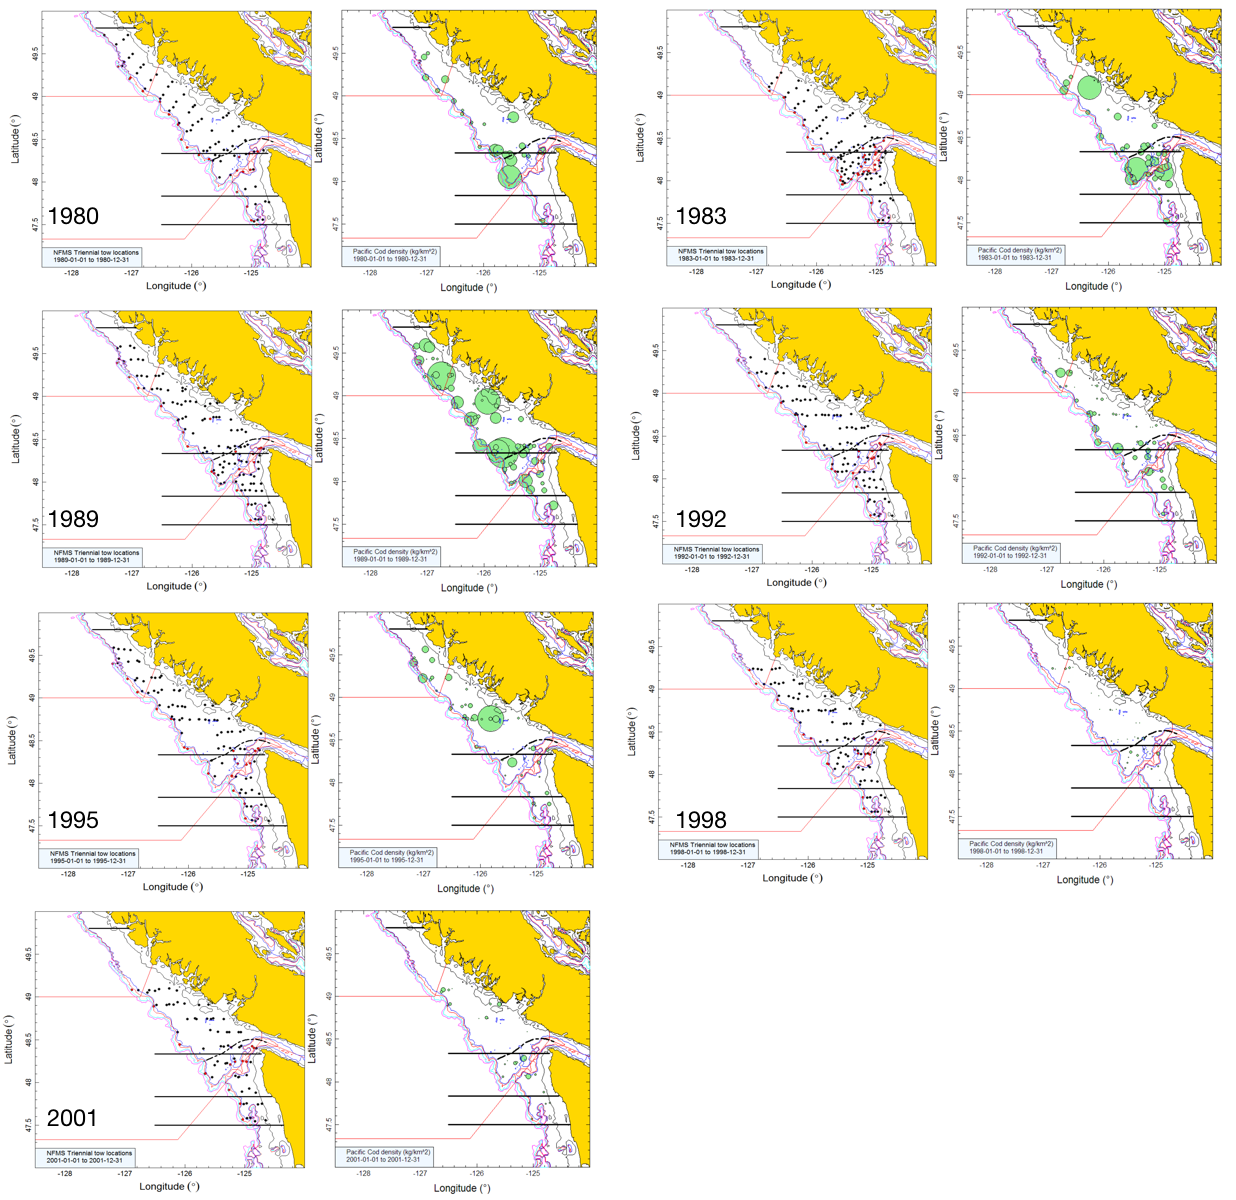
\includegraphics[width=6in]{C:/GitHub/pacific-cod-2020/report/paul-figs/paul-surv-small}}{Figure \ref{fig:tri-tows}} 

}

\caption{(Left panels): plot of tow locations in the Vancouver INPFC region for the NMFS triennial survey in US and Canadian waters. Tow locations are colour-coded by depth range: black=55--183m; red=184-366m; grey=367-500m. Dashed line shows approximate position of the Canada/USA marine boundary. Horizontal lines are the stratum boundaries: 47 30, 47 50, 48 20 and 49 50. Tows south of the 47 30 line were not included in the analysis. (Right panels): circle sizes in the density plot are scaled across all years (1980, 1983, 1989, 1992, 1995, 1998, and 2001), with the largest circle = 7,229 kg/km2 in 1989. The red solid lines indicate the boundaries between PMFC areas 3B, 3C and 3D.}\label{fig:tri-tows}
\end{figure}
\begin{figure}[htb]

{\centering \pdftooltip{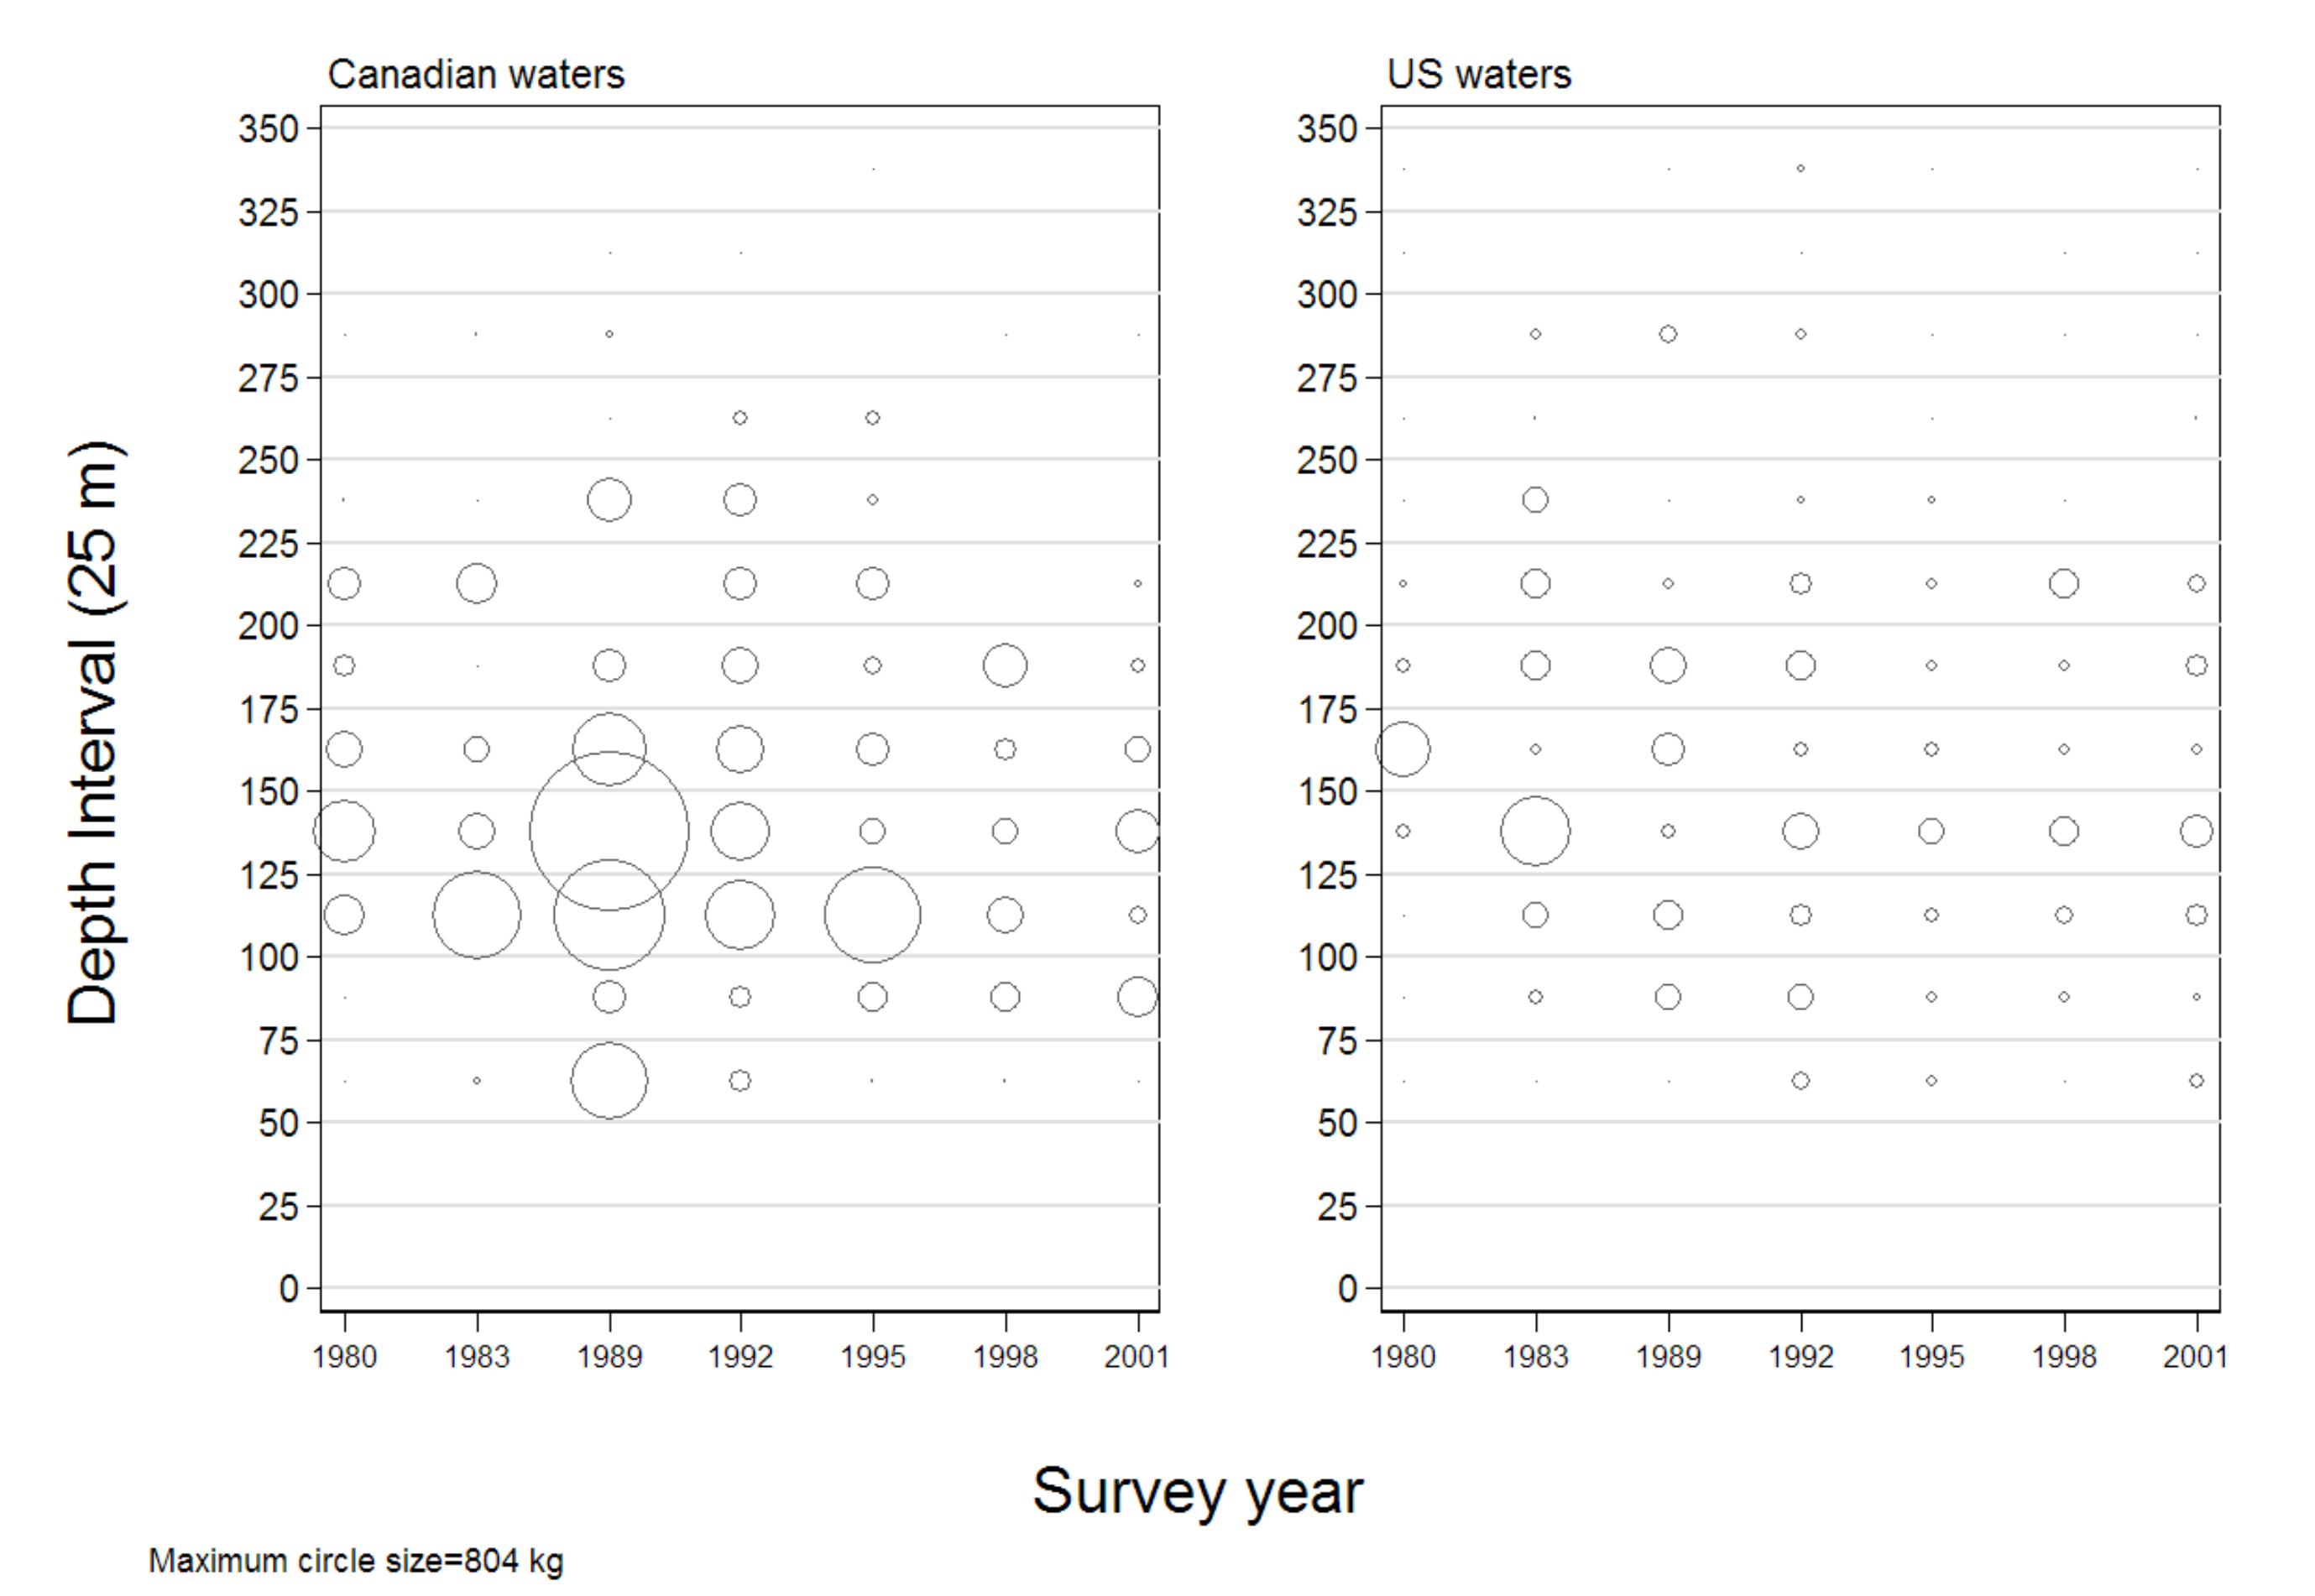
\includegraphics[width=6in]{C:/GitHub/pacific-cod-2020/report/paul-figs/paul8}}{Figure \ref{fig:tri-fig8}} 

}

\caption{Distribution of Pacific Cod catch weights for each survey year summarised into 25 m depth intervals for all tows (Table B.2) in Canadian and US waters of the Vancouver INPFC area. Catches are plotted at the mid-point of the interval.  Note that the deep strata introduced in 1995 (see Table B.2) have been included in this plot but were not used in the biomass estimation.}\label{fig:tri-fig8}
\end{figure}
\begin{figure}[htb]

{\centering \pdftooltip{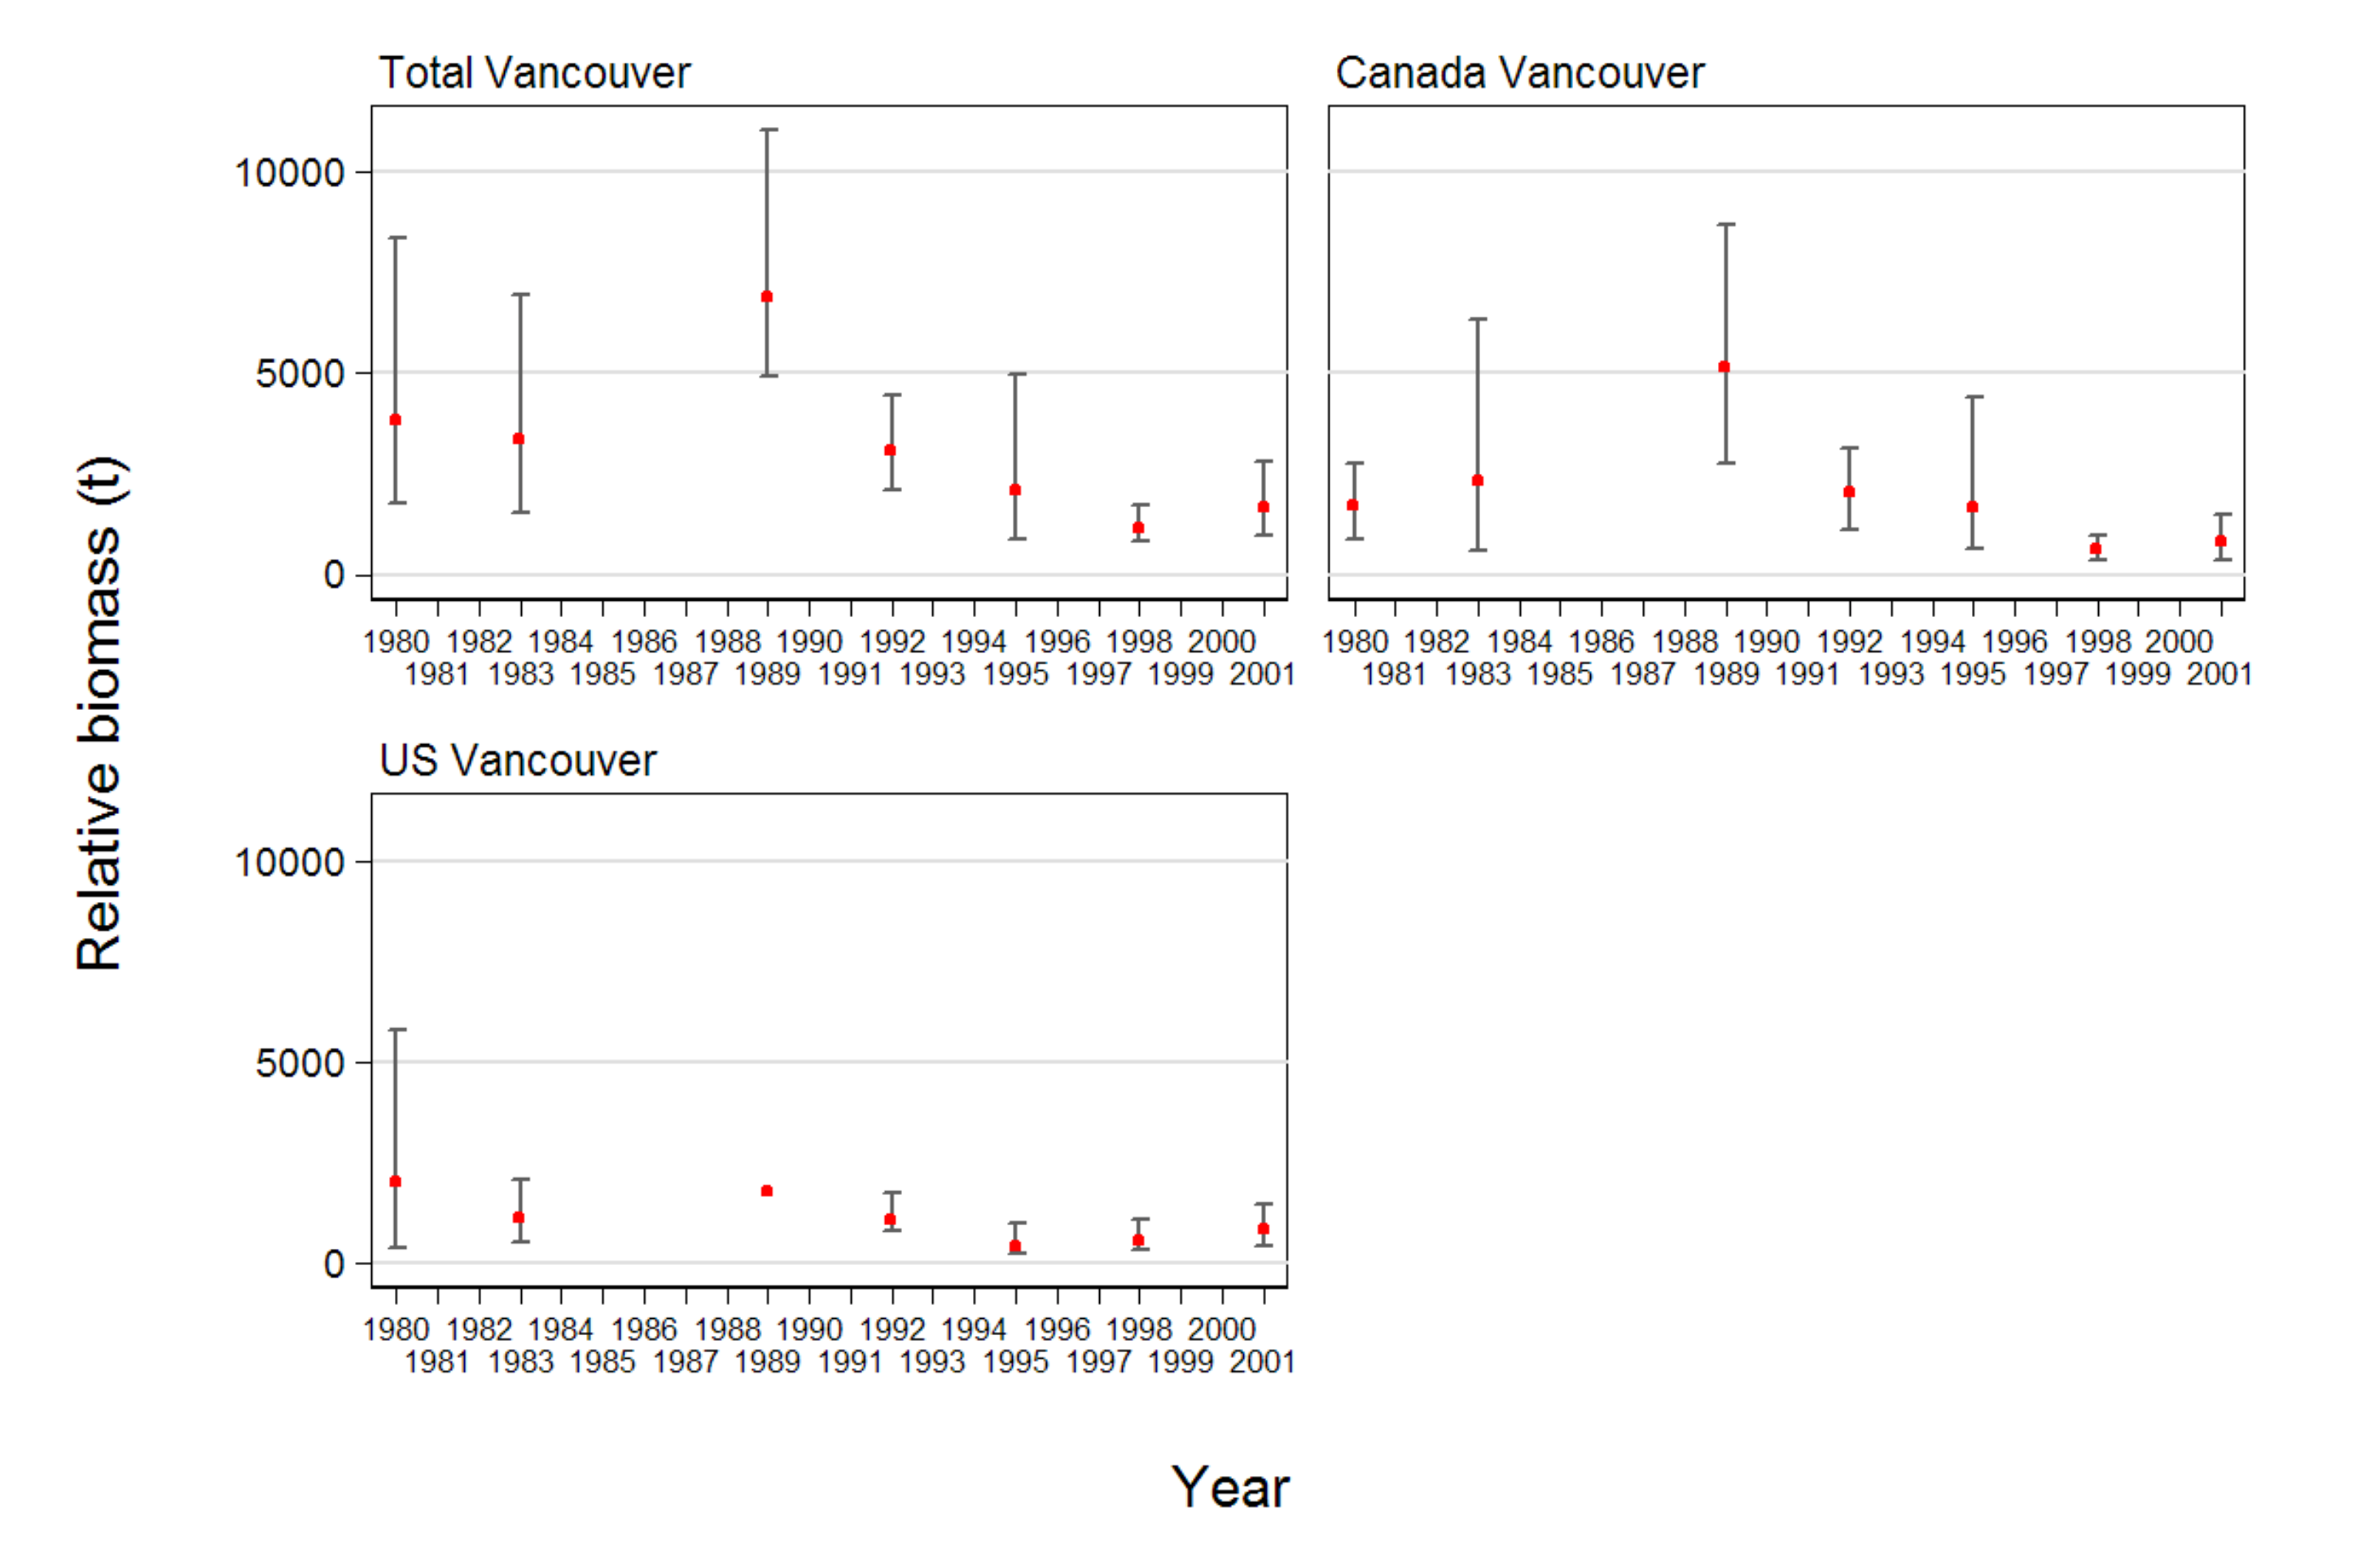
\includegraphics[width=6in]{C:/GitHub/pacific-cod-2020/report/paul-figs/paul9}}{Figure \ref{fig:tri-fig9}} 

}

\caption{Biomass estimates for three series of Pacific Cod in the INPFC Vancouver region (total region, Canadian waters only, US waters only) with 95\% error bars estimated from 1000 bootstraps.}\label{fig:tri-fig9}
\end{figure}
\clearpage

\clearpage

\hypertarget{references}{%
\section*{REFERENCES}\label{references}}
\phantomsection
\addcontentsline{toc}{section}{REFERENCES}
% This manually sets the header for this unnumbered chapter.
\noindent
\vspace{-2em}
\setlength{\parindent}{-0.2in}
\setlength{\leftskip}{0.2in}
\setlength{\parskip}{8pt}

\hypertarget{refs}{}
\leavevmode\hypertarget{ref-choromanski2002}{}%
Choromanski, E.M., Fargo, J., and Kronlund, A.R. 2002. Species assemblage trawl survey of hecate strait, CCGS W.E. RICKER, May 31--June 13, 2000. Can. Data Rep. Fish. Aquat. Sci.: 1085:89.

\leavevmode\hypertarget{ref-efron1982}{}%
Efron, B. 1982. The jackknife, the bootstrap and other resampling plans. SIAM CBMS-NSF Mon. 38: 92.

\leavevmode\hypertarget{ref-fargo1988}{}%
Fargo, J., Foucher, R.P., Saunders, M.W., Tyler, A.V., and Summers, P.L. 1988. 1988 F/V EASTWARD HO Assemblage survey of Hecate Strait, May 27-June 16, 1987. Can. Data Rep. Fish. Aquat. Sci.: 699:172.

\leavevmode\hypertarget{ref-fargo1984}{}%
Fargo, J., Tyler, A.V., Cooper, J., Shields, S.C., and Stebbins, S. 1984. ARCTIC OCEAN Assemblage of Hecate Strait, May 27-June 17, 1984. Can. Data Rep. Fish. Aquat. Sci.: 491:108.

\leavevmode\hypertarget{ref-forrest2020}{}%
Forrest, R.E., Anderson, S.C., Grandin, C.J., and Starr, P.J. 2020. Assessment of Pacific Cod (\emph{Gadus macrocephalus}) for Hecate Strait and Queen Charlotte Sound (Area 5ABCD), and West Coast Vancouver Island (Area 3CD) in 2018. DFO Can. Sci. Advis. Sec. Res. Doc. 2020/nnn(Canadian Science Advisory Secretariat (CSAS) 2020/nnn): nnn.

\leavevmode\hypertarget{ref-hand1994}{}%
Hand, C.M., Robison, B.D., Fargo, J., Workman, G.D., and Stocker, M. 1994. 1994 R/V W.E. RICKER Assemblage survey of Hecate Strait, May 17-June 3, 1993. Can. Data Rep. Fish. Aquat. Sci.: 925:197.

\leavevmode\hypertarget{ref-sinclair2000}{}%
Sinclair, A.F. 1999. Survey design considerations for Pacific cod in Hecate Strait. DFO Can. Sci. Advis. Sec. Res. Doc. 196: 42 p.

\leavevmode\hypertarget{ref-sinclair2001}{}%
Sinclair, A.F., Martell, S., and Boutillier, J. 2001. Assessment of Pacific Cod off the West Coast of Vancouver Island and in Hecate Strait, Nov. 2001. DFO Can. Sci. Advis. Sec. Res. Doc. 159: 61 p.

\leavevmode\hypertarget{ref-sinclair2005}{}%
Sinclair, A.F., and Starr, P.J. 2005. Assessment of Pacific Cod in Hecate Strait (5CD) and Queen Charlotte Sound (5AB), January 2005. DFO Can. Sci. Advis. Sec. Res. Doc. 026: 97 p.

\leavevmode\hypertarget{ref-sinclair2007}{}%
Sinclair, A., Krishka, B.A., and Fargo, J. 2007. Species trends in relative biomass, occupied area and depth distribution for Hecate Strait Assemblage Surveys from 1984-2003. Can. Tech Rep. Fish. Aquat. Sci.: 2749:141.

\leavevmode\hypertarget{ref-westrheim1984}{}%
Westrheim, S.J., Tyler, A.V., Foucher, R.P., Saunders, M.W., and Shields, S.C. 1984. G.B. Reed Groundfish Cruise No. 84-3, May 24-June 14, 1984. Can. Data Rep. Fish. Aquat. Sci.: 131.

\leavevmode\hypertarget{ref-wilson1991}{}%
Wilson, S.J., Fargo, J., Hand, C.M., Johansson, T., and Tyler, A.V. 1991. 1991 R/V W.E. RICKER Assemblage survey of Hecate Strait, June 3-22, 1991. Can. Data Rep. Fish. Aquat. Sci.: 866:179.

\leavevmode\hypertarget{ref-workman1997}{}%
Workman, G.D., Fargo, J., Beall, B., and Hildebrandt, E. 1997. 1997 R/V W.E. RICKER Assemblage survey of Hecate Strait, May 30-June 13, 1996. Can. Data Rep. Fish. Aquat. Sci.: 1010:155.

\leavevmode\hypertarget{ref-workman1996}{}%
Workman, G.D., Fargo, J., Yamanaka, K.L., and Haist, V. 1996. 1996 R/V W.E. RICKER Assemblage survey of Hecate Strait, May 23-June 9, 1995. Can. Data Rep. Fish. Aquat. Sci.: 974:94.

\setlength{\parindent}{0in} \setlength{\leftskip}{0in} \setlength{\parskip}{4pt}

\markboth{References}{References}

\end{document}
